\section{Técnica Proposta}
\subsection*{}

% apresenta dod
% apresenta padrão entity system
% apresenta implementações
% apresenta os 3 problemas que serão tratados


\begin{frame}{Organização dos dados proposta}

    \vspace{1cm}

    \begin{itemize}
        \item \textbf{Data-Oriented Design} (DOD)
        \begin{itemize}
            \item Focado na organização dos dados
            \item Otimização do uso da memória cache
        \end{itemize}
        \item \textbf{Entity-Component System} (ECS)
        \begin{itemize}
            \item \textbf{Padrão de projeto} utilizado principalmente no desenvolvimento de jogos
            \item Baseado em \textbf{Entidades} e \textbf{Propriedades} (Componentes)
        \end{itemize}
    \end{itemize}

    \pgfdeclareimage[width=0.4\linewidth]{entity}{img/tecnica/entity.pdf}
    % \pgfdeclareimage[width=0.7\linewidth]{entity_pin}{img/tecnica/pin_dod.pdf}

    \begin{center}
        \pgfuseimage<1>{entity}
        % \pgfuseimage<2>{entity_pin}
    \end{center}

\end{frame}

\begin{frame}{Organização dos dados proposta}
    \begin{columns}
        \column{.45\linewidth}
            \pgfdeclareimage[width=\linewidth]{fig1}{img/tecnica/registerClusterclassOOD.pdf}
            \begin{itemize}
                \item Object-Oriented Design
            \end{itemize}
            \pgfuseimage<1>{fig1}
        \column{.5\linewidth}
            \pgfdeclareimage[width=\linewidth]{fig2}{img/tecnica/propertiesDOD.pdf}
            \begin{itemize}
                \item Data-Oriented Design
            \end{itemize}
            \pgfuseimage<1>{fig2}
    \end{columns}
\end{frame}




\begin{frame}{Operações: busca, adição, e remoção de entidades em $\mathcal{O}(1)$}

\pgfdeclareimage[width=0.9\linewidth]{es1}{img/tecnica/entitySystemInsertion_1.pdf}
\pgfdeclareimage[width=0.9\linewidth]{es2}{img/tecnica/entitySystemInsertion_2.pdf}
\pgfdeclareimage[width=0.7\linewidth]{es3}{img/tecnica/entitySystemInsertion_3.pdf}
\pgfdeclareimage[width=0.7\linewidth]{es31}{img/tecnica/entitySystemInsertion_3_1.pdf}
\pgfdeclareimage[width=0.7\linewidth]{mask}{img/tecnica/mask.pdf}

\only<1>{
    \begin{itemize}
        \item \textbf{Busca}: $\mathcal{O}(1)$
    \end{itemize}
    \begin{center}
        \pgfuseimage{es1}
    \end{center}
}
\only<2>{
    \begin{itemize}
        \item \textbf{Adição}: $\mathcal{O}(1)$
    \end{itemize}
    \begin{center}
        \pgfuseimage{es2}
    \end{center}
}
\only<3>{
    \vspace{0.5cm}
    \begin{itemize}
        \item \textbf{Remoção}: $\mathcal{O}(1)$
    \end{itemize}
    \vspace{-0.5cm}
    \begin{center}
        \pgfuseimage{es31}
        
        \vspace{0.5cm}
        
        \pgfuseimage{mask}
    \end{center}
}
\only<4>{
    \vspace{0.5cm}
    \begin{itemize}
        \item \textbf{Remoção}: $\mathcal{O}(1)$
    \end{itemize}
    \vspace{-0.5cm}
    \begin{center}
        \pgfuseimage{es31}
        
        \vspace{0.5cm}
        
        \pgfuseimage{es3}
    \end{center}
}

% \begin{center}
    % \pgfuseimage<1>{es1}
    % \pgfuseimage<2>{es2}
    % \pgfuseimage<3>{es3}
% \end{center}

\end{frame}

% \begin{frame}{Relationships Between Entities: aggregation and composition}

% \pgfdeclareimage[width=0.75\linewidth]{es1}{img/tecnica/aggregation_composition_1.pdf}
% \pgfdeclareimage[width=0.75\linewidth]{es2}{img/tecnica/aggregation_composition_2.pdf}
% \pgfdeclareimage[width=0.75\linewidth]{es3}{img/tecnica/aggregation_composition_3.pdf}
% \pgfdeclareimage[width=0.75\linewidth]{es4}{img/tecnica/aggregation_composition_4.pdf}

% \vspace{10pt}

% \begin{center}

% \pgfuseimage<1>{es1}
% \pgfuseimage<2>{es2}
% \pgfuseimage<3>{es3}
% \pgfuseimage<4>{es4}

% \end{center}

% \end{frame}

% \begin{frame}{Aggregation code example}

    
%     \begin{figure}
%         \centering
%         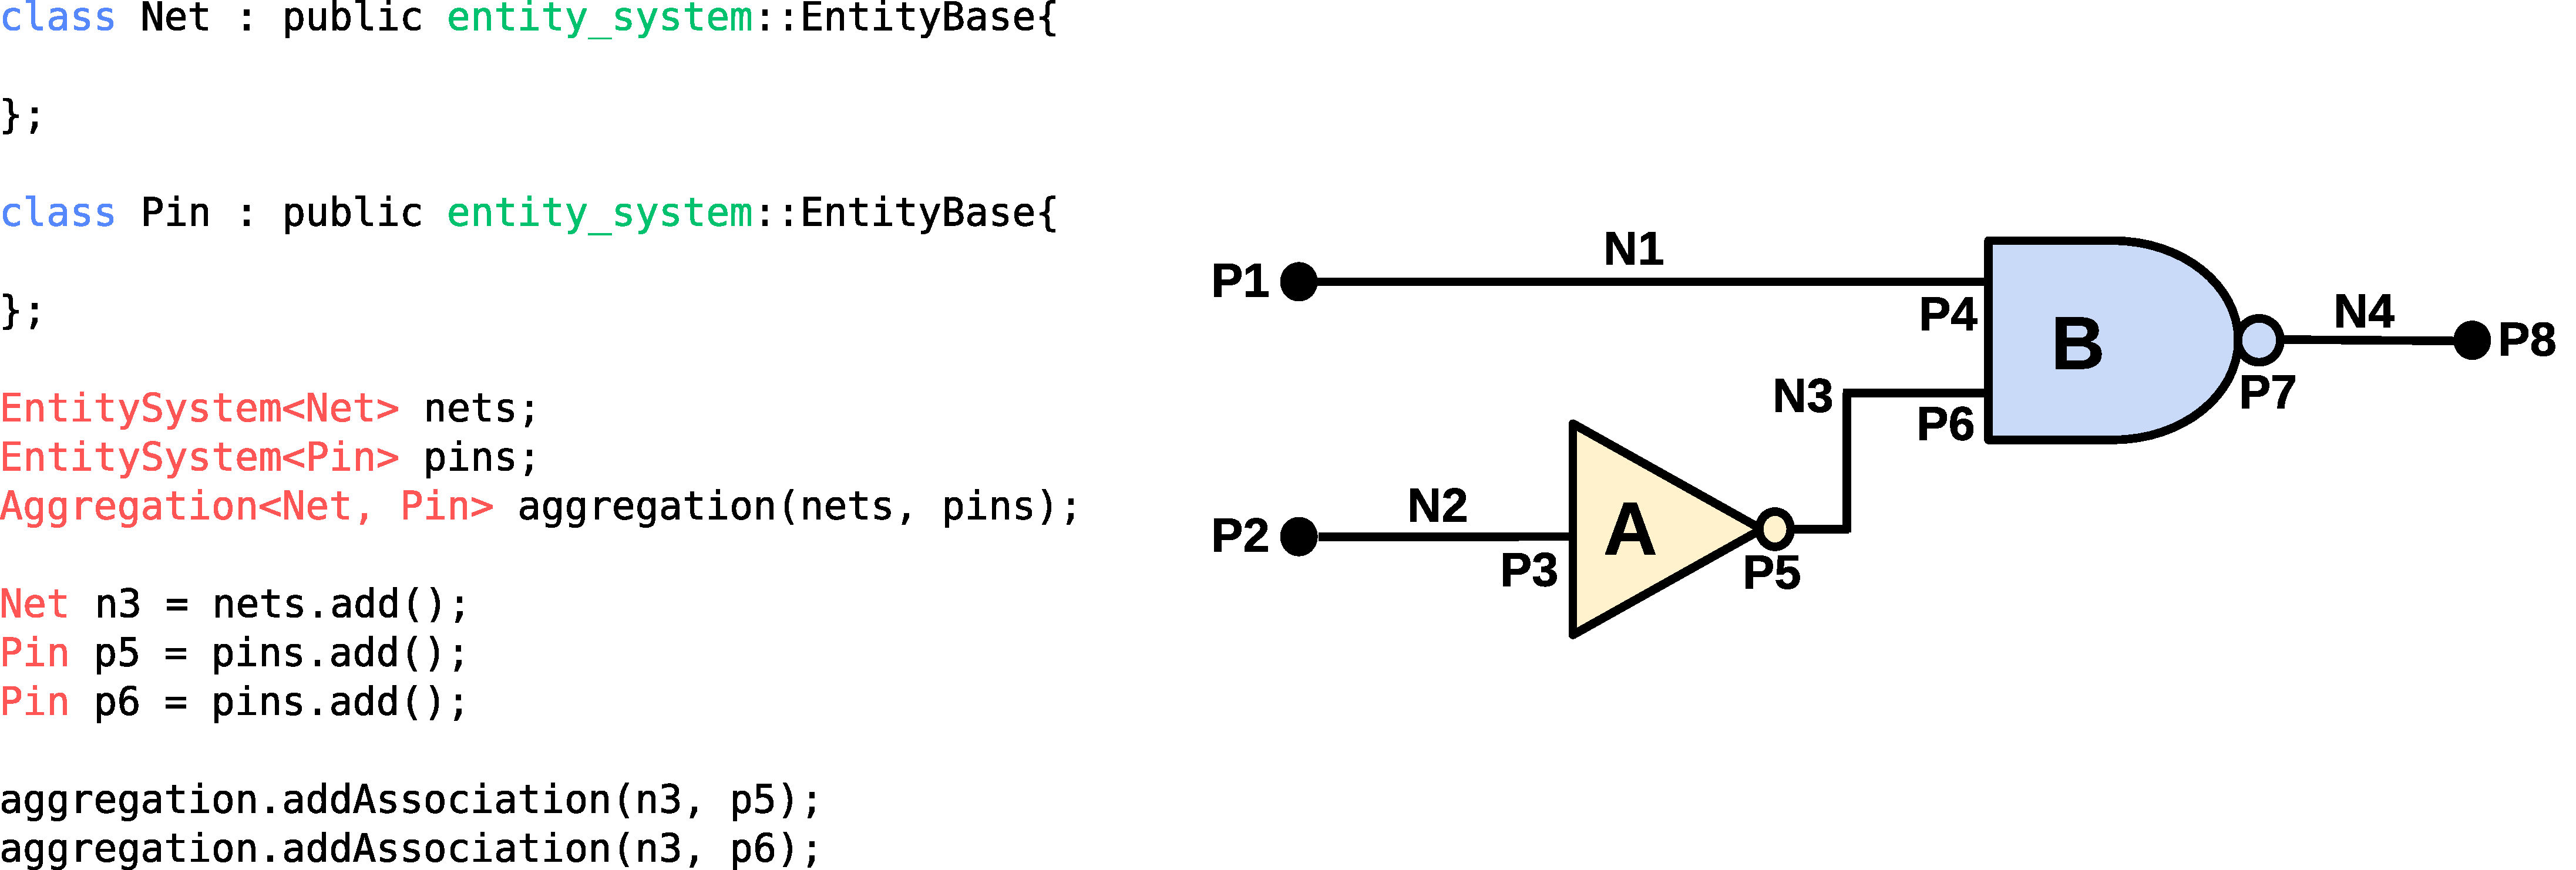
\includegraphics[width=\textwidth]{img/tecnica/code_example_aggregation.pdf}
%     \end{figure}

% \end{frame}

% \begin{frame}{Composition code example}

    
%     \begin{figure}
%         \centering
%         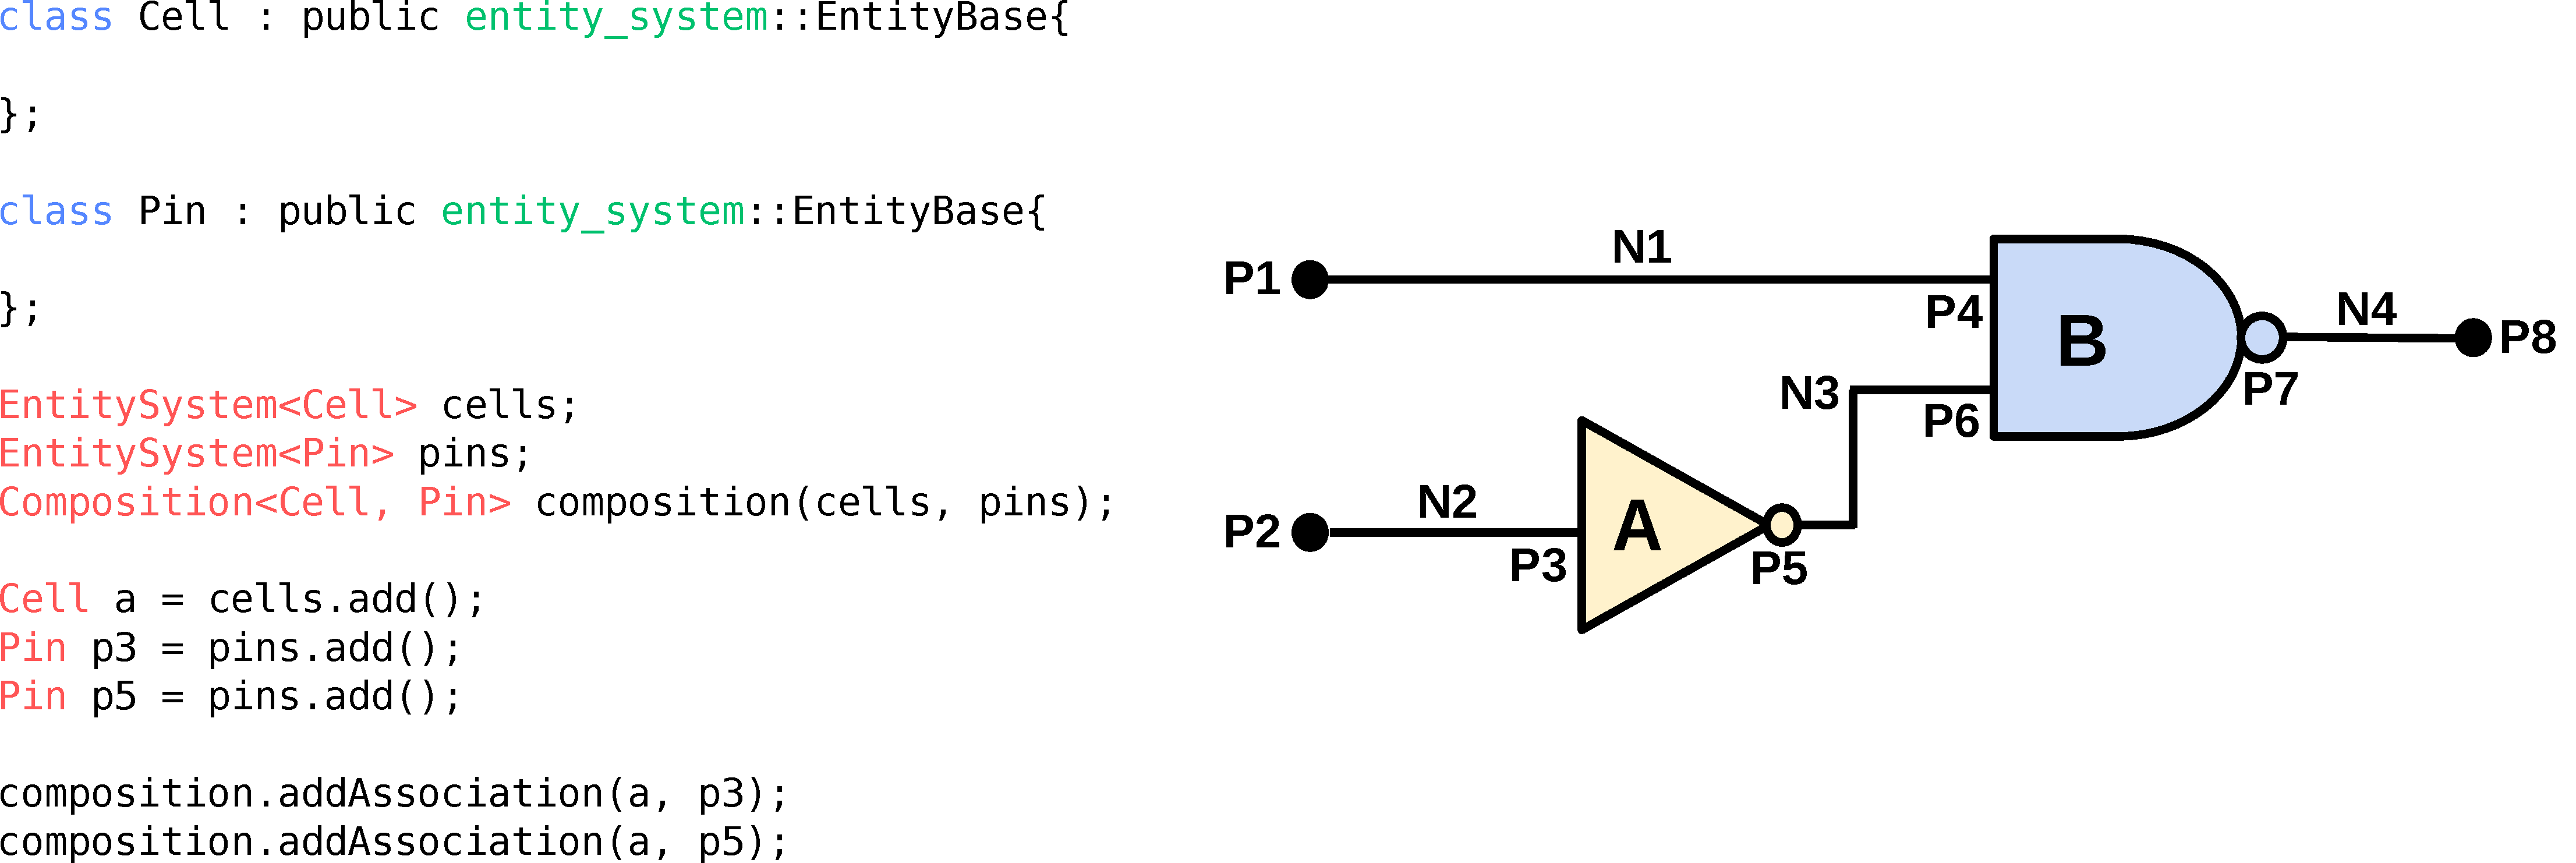
\includegraphics[width=\textwidth]{img/tecnica/code_example_composition.pdf}
%     \end{figure}

% \end{frame}


% ---------------------------------------------------------------------------------------------------------
